\documentclass{beamer}

\usetheme{default}

\usepackage{subcaption}
\usepackage{graphicx}
\begin{document}

\title{Quick results}
\author{Pierre Marrec}
\date{\today}

\begin{frame}
    \titlepage
\end{frame}

\begin{frame}
    \frametitle{Introduction}


    Rappel des données
   \begin{itemize}
    \item 1 athlètes (15600)
    \item de juin 2020 à avril 2024 (on a des données à partir de 2019 mais pas de RPE)
    \item piste, route, clm, home trainer
    \item nettoyage : suppression des séquences sans données $>$ 5min, interpolation au maximum, suppression des séquences avec des valeurs aberrantes, séance trop courtes (négatives,trop basses, trop hautes etc.)
   \end{itemize}
    \begin{table}
        \centering
        \begin{tabular}{|c|c|c|c|}
            \hline
            etat & nombre de points & nombres de séances \\
            \hline
            complète & 9440286 & 1534 \\
            nettoyée & 4239646& 715\\
            \hline
        \end{tabular}
    \end{table}

    %problème avec uniquement la puissance
    %Rolling -> graph ppr and ma_hr
    % Impact du rolling mean sur les données

    % Time with Power and RPE
    % Time with Power and HR -> PAs tellement mieux
    % Time with HR and RPE -> Bien mieux

    % Power for each state based on HR -> show a progression

\end{frame}

\begin{frame}{La dernière fois}
    \begin{figure}
        \begin{subfigure}{0.35\textwidth}
            \includegraphics[width=\textwidth]{figures/time_no_roll.png}
            \caption{Proportion du temps passé dans chaque état}
        \end{subfigure}
        \begin{subfigure}{0.6\textwidth}
            \includegraphics[width=\textwidth]{figures/sequence.png}
            \caption{Labelisation des séquences}
        \end{subfigure}
        
    \end{figure}
\end{frame}



\begin{frame}{Impact de la normalisation par la PPR des 2 derniers mois}
    \begin{figure}
        \begin{subfigure}{0.45\textwidth}
            \centering
            \includegraphics[width=\textwidth]{figures/time_no_roll.png}
            \caption{Normalisation sur toute la période}
            
        \end{subfigure}
        \begin{subfigure}{0.45\textwidth}
            \centering
            \includegraphics[width=\textwidth]{figures/time_roll.png}
            \caption{Normalisation sur les 2 derniers mois}
        \end{subfigure}
    \end{figure}
\end{frame}
\begin{frame}{PPR mobile et moyenne mobile de la fréquence cardiaque}
    \begin{figure}
        \centering
        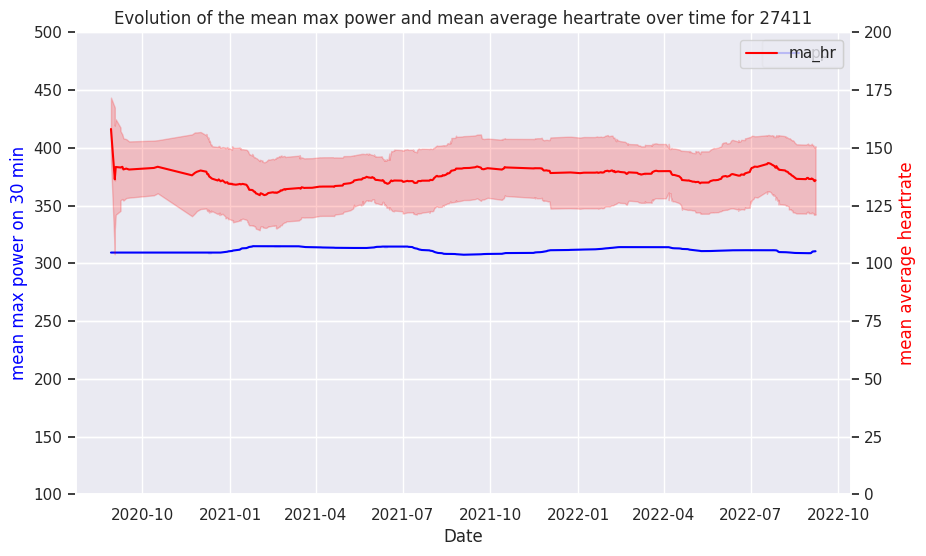
\includegraphics[width=0.8\textwidth]{figures/ppr_ma_hr.png}
        \caption{PPR mobile et moyenne mobile de la fréquence cardiaque}
    \end{figure}
\end{frame}

\begin{frame}{Rajoute la fréquence cardiaque}
    \begin{figure}
        \begin{subfigure}{0.45\textwidth}
            \centering
            \includegraphics[width=\textwidth]{figures/time_roll.png}
            \caption{Etat appris que sur la puissance normalisée}
        \end{subfigure}
        \begin{subfigure}{0.45\textwidth}
            \centering
            \includegraphics[width=\textwidth]{figures/time_hr_power.png}
            \caption{État appris avec la puissance et la fréquence cardiaque normalisée}
        \end{subfigure}
    \end{figure}    
\end{frame}

\begin{frame}{Avec la fréquence cardiaque uniquement}
    \begin{figure}
        \begin{subfigure}{0.45\textwidth}
            \centering
            \includegraphics[width=\textwidth]{figures/time_hr_power.png}
            \caption{État appris avec la puissance et la fréquence cardiaque normalisée}
        \end{subfigure}
        \begin{subfigure}{0.45\textwidth}
            \centering
            \includegraphics[width=\textwidth]{figures/time_hr.png}
            \caption{État appris avec la fréquence cardiaque normalisée}
        \end{subfigure}
    \end{figure}
\end{frame}

\begin{frame}{Matrice de transition et fréquence cardiaque moyenne par état}
    \begin{figure}
        \begin{subfigure}{0.4\textwidth}
            \centering
            \includegraphics[width=0.8\textwidth]{figures/matrix_final.pdf}
            \caption{Matrice de transition}
        \end{subfigure}
        \begin{subfigure}{0.55\textwidth}
            \centering
            \includegraphics[width=0.8\textwidth]{figures/box_final}
            \caption{Fréquence cardiaque moyenne par état au cours du temps}
        \end{subfigure}
    \end{figure}
\end{frame}

\begin{frame}{Puissance moyenne par état cardiaque}
    \begin{figure}
        \centering
        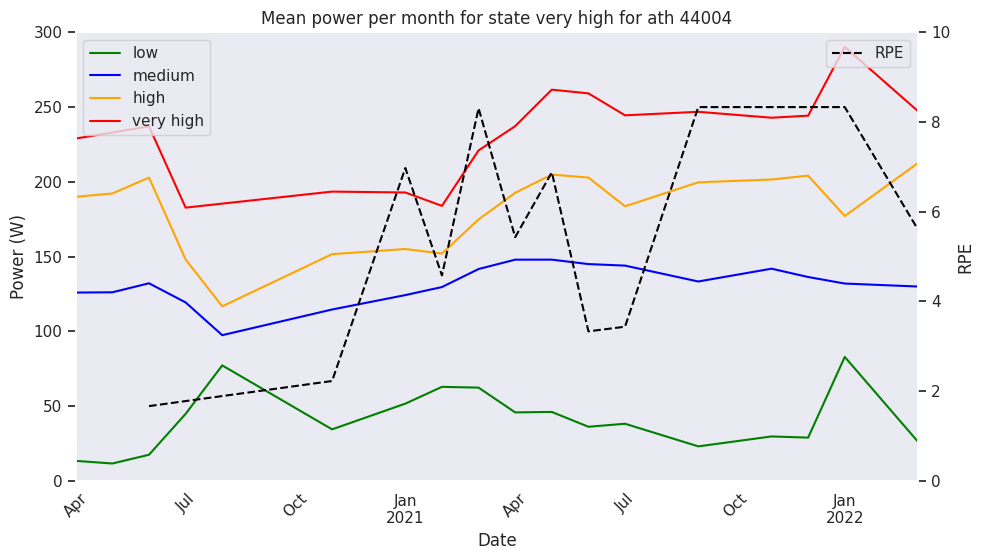
\includegraphics[width=0.8\textwidth]{figures/4_states_roll_all.png}
        \caption{Puissance moyenne par état au cours du temps}
    \end{figure}
\end{frame}
\begin{frame}{Zoom sur les états}
    %subfigure of 4
    \begin{figure}
        \centering
        \begin{subfigure}{0.45\textwidth}
            \centering
            \includegraphics[width=\textwidth]{figures/4_states_roll_low.png}
            \caption{low}
        \end{subfigure}
        \begin{subfigure}{0.45\textwidth}
            \centering
            \includegraphics[width=\textwidth]{figures/4_states_roll_medium.png}
            \caption{medium}
        \end{subfigure}
        \begin{subfigure}{0.45\textwidth}
            \centering
            \includegraphics[width=\textwidth]{figures/4_states_roll_high.png}
            \caption{high}
        \end{subfigure}
        \begin{subfigure}{0.45\textwidth}
            \centering
            \includegraphics[width=\textwidth]{figures/4_states_roll_very high.png}
            \caption{very high}
        \end{subfigure}
        \caption*{Puissance moyenne par état au cours du temps avec régression linéaire}
    \end{figure}
\end{frame}
\begin{frame}{Puissance max et fréquence moyenne}
    \begin{figure}
        \centering
        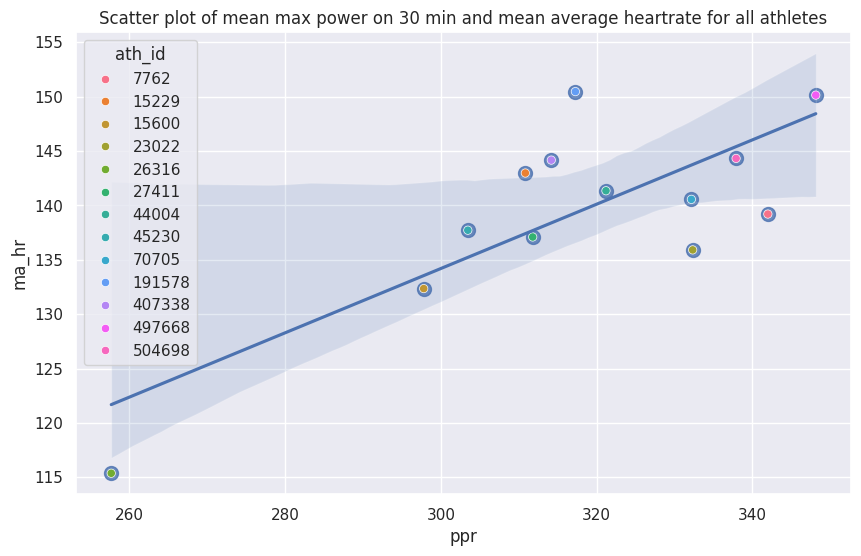
\includegraphics[width=0.9\textwidth]{figures/ppr_ma_hr_all_ath}
        \caption{Puissance max et fréquence cardiaque moyenne pour tous les athlètes}
    \end{figure}
\end{frame}

\begin{frame}{Zoom sur les états}
    %subfigure of 4
    \begin{figure}
        \centering
        \begin{subfigure}{0.45\textwidth}
            \centering
            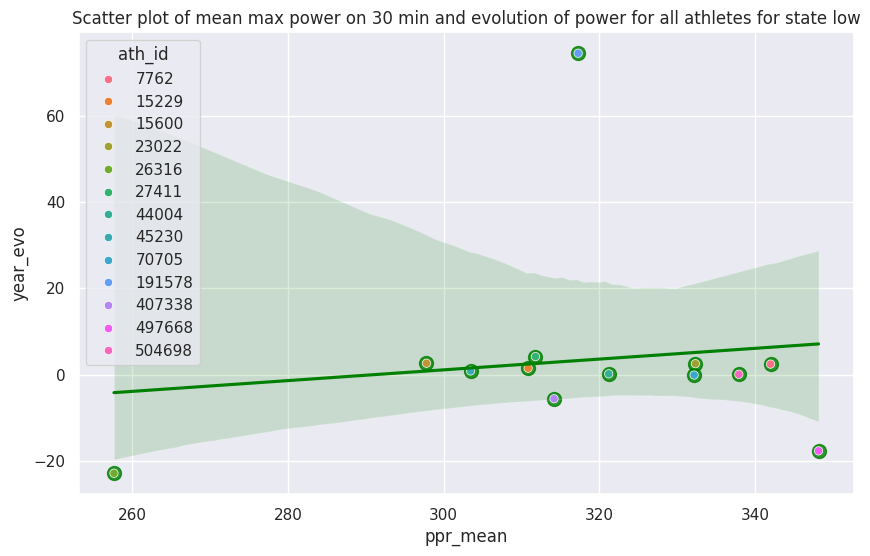
\includegraphics[width=\textwidth]{figures/evolution_power_ppr_low.png}
            \caption{low}
        \end{subfigure}
        \begin{subfigure}{0.45\textwidth}
            \centering
            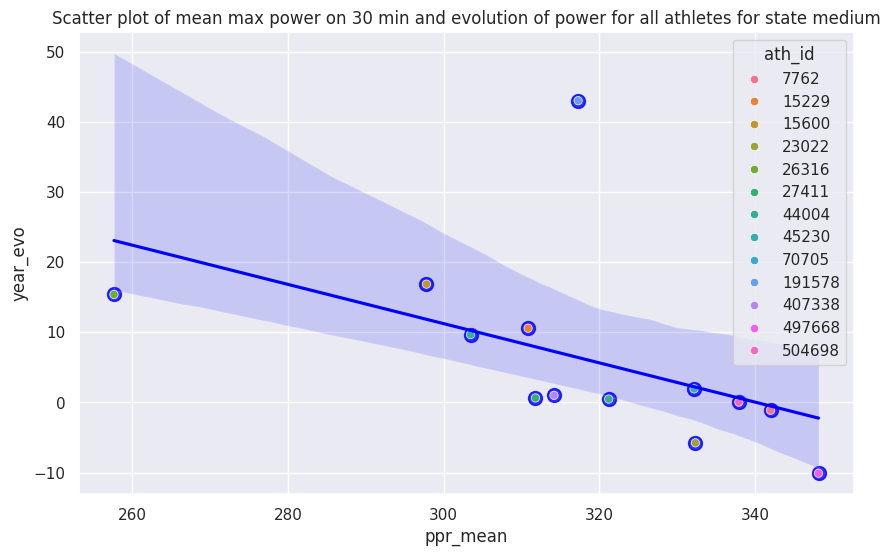
\includegraphics[width=\textwidth]{figures/evolution_power_ppr_medium.png}
            \caption{medium}
        \end{subfigure}
        \begin{subfigure}{0.45\textwidth}
            \centering
            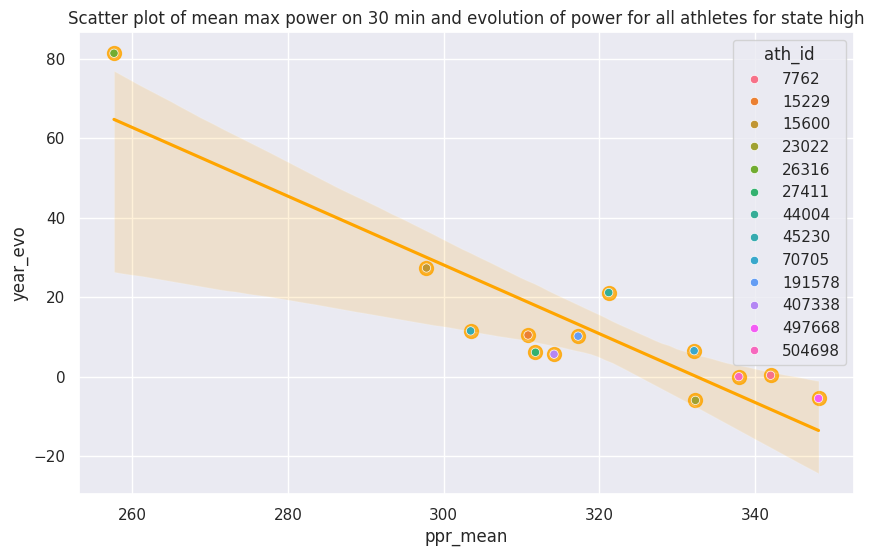
\includegraphics[width=\textwidth]{figures/evolution_power_ppr_high.png}
            \caption{high}
        \end{subfigure}
        \begin{subfigure}{0.45\textwidth}
            \centering
            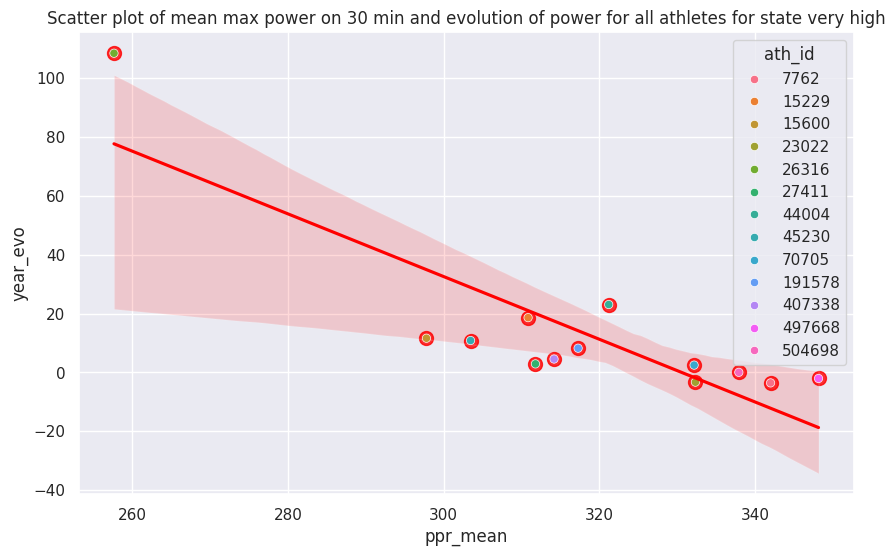
\includegraphics[width=\textwidth]{figures/evolution_power_ppr_very high.png}
            \caption{very high}
        \end{subfigure}
        \caption*{Répartition des athlètes dans en fonction de la PPR et de l'évolution des la puissances pour les différents états}
    \end{figure}
\end{frame}
\begin{frame}{Zoom sur les états}
    %subfigure of 4
    \begin{figure}
        \centering
        \begin{subfigure}{0.45\textwidth}
            \centering
            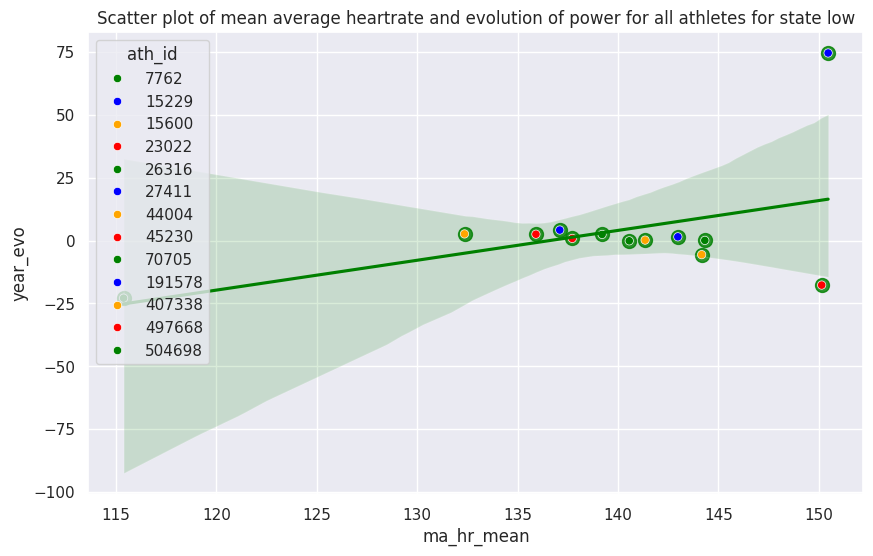
\includegraphics[width=\textwidth]{figures/evolution_power_ma_low.png}
            \caption{low}
        \end{subfigure}
        \begin{subfigure}{0.45\textwidth}
            \centering
            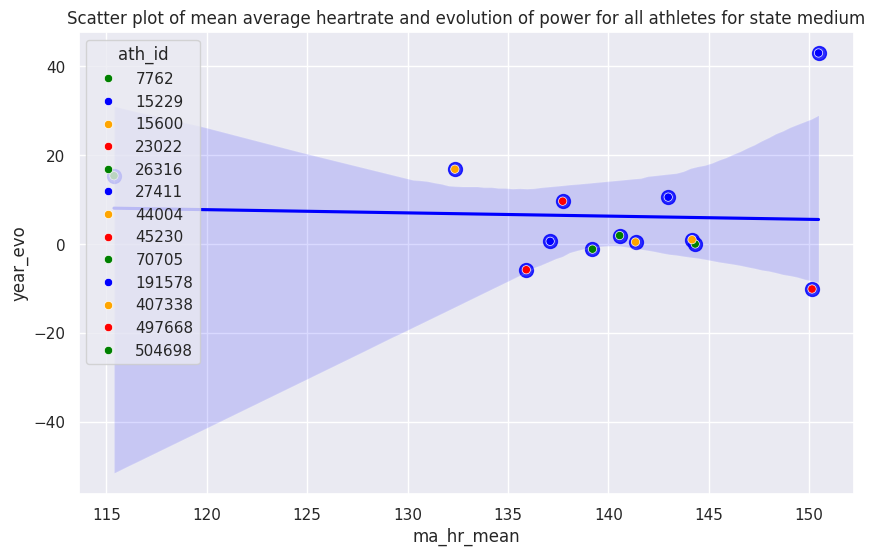
\includegraphics[width=\textwidth]{figures/evolution_power_ma_medium.png}
            \caption{medium}
        \end{subfigure}
        \begin{subfigure}{0.45\textwidth}
            \centering
            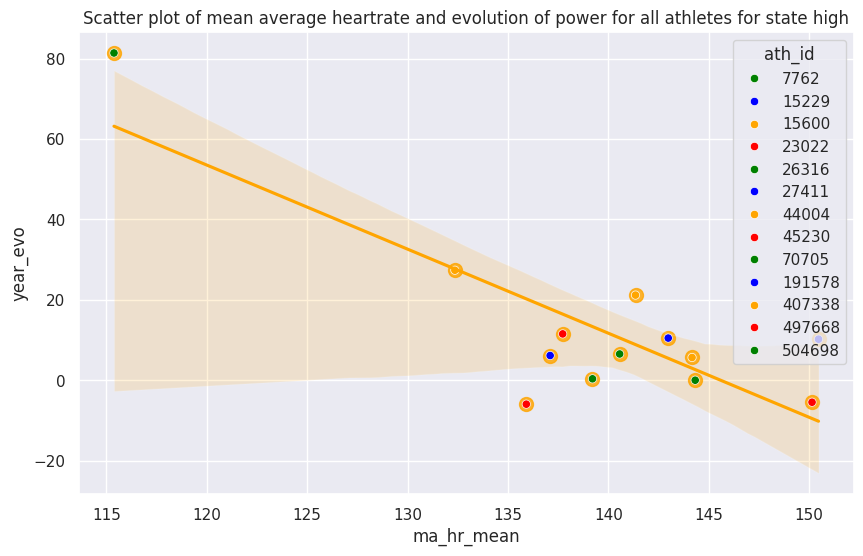
\includegraphics[width=\textwidth]{figures/evolution_power_ma_high.png}
            \caption{high}
        \end{subfigure}
        \begin{subfigure}{0.45\textwidth}
            \centering
            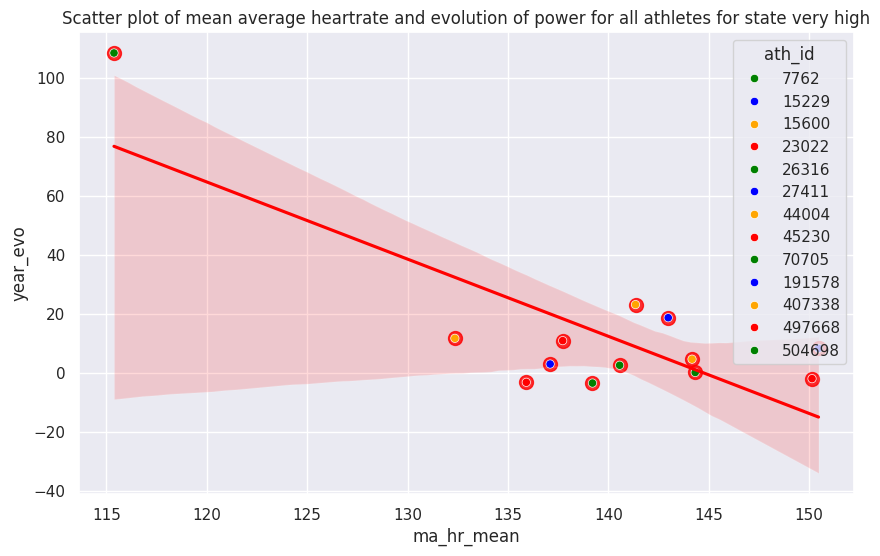
\includegraphics[width=\textwidth]{figures/evolution_power_ma_very high.png}
            \caption{very high}
        \end{subfigure}
        \caption*{Répartition des athlètes dans en fonction de la fréquence moyenne et de l'évolution des la puissances pour les différents états}
    \end{figure}
\end{frame}




\begin{frame}{La suite}
    \begin{itemize}
        \item Comparer aux modèles par athlètes
        \item Estimer l'évolution de la puissance moyenne par état
        \item Utiliser les états et la puissance par état pour décrire
    \end{itemize}
\end{frame}



\end{document}